\documentclass[tikz,border=10pt]{standalone}
\usepackage{amsmath}
\usepackage{bm}
\usetikzlibrary{arrows.meta,decorations.pathmorphing}

% ---- Muted academic theme ----
\definecolor{slate}{HTML}{2C3E50}
\definecolor{oiblue}{HTML}{0072B2}
\definecolor{oiorange}{HTML}{E69F00}
\definecolor{oigreen}{HTML}{009E73}
\definecolor{oivermil}{HTML}{D55E00}

% ---- SCHEMATIC KIT: the Riemann fan, both frames ------------------
% THIS FIGURE IS A CARTOON.  Unlike every other kit in this set it is NOT
% drawn to scale and does NOT correspond to any solved problem -- deliberately,
% because its job is to show the STRUCTURE before any wave type is chosen.
% Line art only, no pressure-tracking region fills, so that it reads as
% different in kind from the to-scale figures.
%
% THE WEDGE DEVICE.  Each outer wave is drawn as a TINTED WEDGE bounded by two
% rays, not as a line and not as a pair of lines.  The tint is what makes it
% one object: a wave whose TYPE is not yet specified.  Open the wedge and it is
% a rarefaction fan; close it to zero width and it is a shock.  One picture
% therefore covers shock/shock, shock/rarefaction, rarefaction/shock and
% rarefaction/rarefaction.  The legend below the panels states the convention.
% Labelling the wedge ONCE, in its middle, is essential -- labelling both edges
% invites the reader to count five waves instead of three.
%
% THE TWO PANELS are the same event in two frames:
%   (a) t-x, Eulerian.  lambda = u-a, u, u+a.  The contact is SLANTED at
%       slope 1/u*, and the whole pattern is skewed downstream by advection.
%   (b) t-h, Lagrangian.  lambda = -Z, 0, +Z.  The contact is VERTICAL, and
%       advection has been transformed away, so the pattern straddles the axis.
% The vertical contact in (b) is the one EXACT claim this cartoon makes; the
% slopes themselves are illustrative.
%
% Cartoon speeds (chosen for legibility, not solved):
%   (a) dx/dt : -1.20 -> -0.75 | contact +0.40 | +1.35 -> +1.70
%   (b) dh/dt : -1.35 -> -1.00 | contact  0.00 | +1.00 -> +1.35
% Windows are both 4.05 units wide so the panels sit at identical scale:
%   (a) x = [-1.85, 2.20]   (b) h = [-2.025, 2.025]   both t = [0, 1.15]
% ---- v3 CHANGES (from DK's edited version) ---------------------------
% 1. t-SCALE 3.2 cm per unit (was 5.2).  The fan looked tall and skinny
%    because the vertical scale was 3.1x the horizontal, so a unit-speed wave
%    drew at 72 deg.  Speeds are UNCHANGED -- region widths at a given t are set
%    by the speeds alone, so pushing the waves outward would only squeeze U_L
%    and U_R off the frame.  The aspect ratio is the only free lever.  Wedge
%    edges now sit at (a) head 57.8 / tail 68.5, (b) head 54.7 / tail 62.3 deg.
% 2. WAVE LABELS are now short tags (lambda_1, lambda_2, lambda_3) beside each
%    wave, with the DEFINITIONS moved to a line under each panel title.  At
%    normalsize the full 'lambda_1 = u_p - c_s' needs about 2.4 cm of vertical
%    run and the panel is only 3.68 cm tall, so it could not sit on the
%    wave.  Side effect worth keeping: the two definition lines now sit side by
%    side, so u_p +- c_s -> +-Z and u_p -> 0 reads straight off the page.
% 3. All rotations recomputed against the edge each tag now sits beside.
% 5. Slope note dropped from -2.02 to -2.40 cm for breathing room under the
%    lambda definition lines; legend block follows to -4.68, which also restores its own clearance.
% 4. SLOPE CONVENTION stated on the figure.  lambda_i is a wave SPEED, dx/dt or
%    dh/dt; because t is the ordinate, the slope actually drawn is 1/lambda_i --
%    the same 'all slopes are inverse velocities' convention as the U6 t-x
%    diagrams.  Kept as a single line rather than per-wave callouts: the
%    definitions must stay as lambda_i because that is what the characteristic
%    form, the CFL condition and the eigenvectors all use.  Bonus: it makes the
%    vertical contact quantitative, since 1/lambda_2 -> infinity when lambda_2 = 0.
% The normalsize fonts, u_p +- c_s notation, low/high region-label split and
% 'indicates' wording are preserved from the edited version.
%
% Scales: 1.68 cm per unit abscissa, 3.2 cm per unit t.  Panel width 6.80 cm,
% panel gap 1.50 cm, so panel (b) is offset by 8.30 cm.
\tikzset{
  axis/.style   = {-{Stealth[length=6pt]}, slate, thin},
  edgeL/.style  = {oiblue, line width=1.2pt},
  edgeR/.style  = {oiorange, line width=1.2pt},
  contact/.style= {slate, line width=1.3pt},
  reg/.style    = {font=\normalsize, text=slate},
  wlab/.style   = {font=\normalsize\sffamily, text=slate, inner sep=2.5pt},
  sweep/.style  = {{Stealth[length=5pt]}-{Stealth[length=5pt]}, slate, thin},
  panel/.style  = {font=\normalsize\bfseries, text=slate},
}

\begin{document}
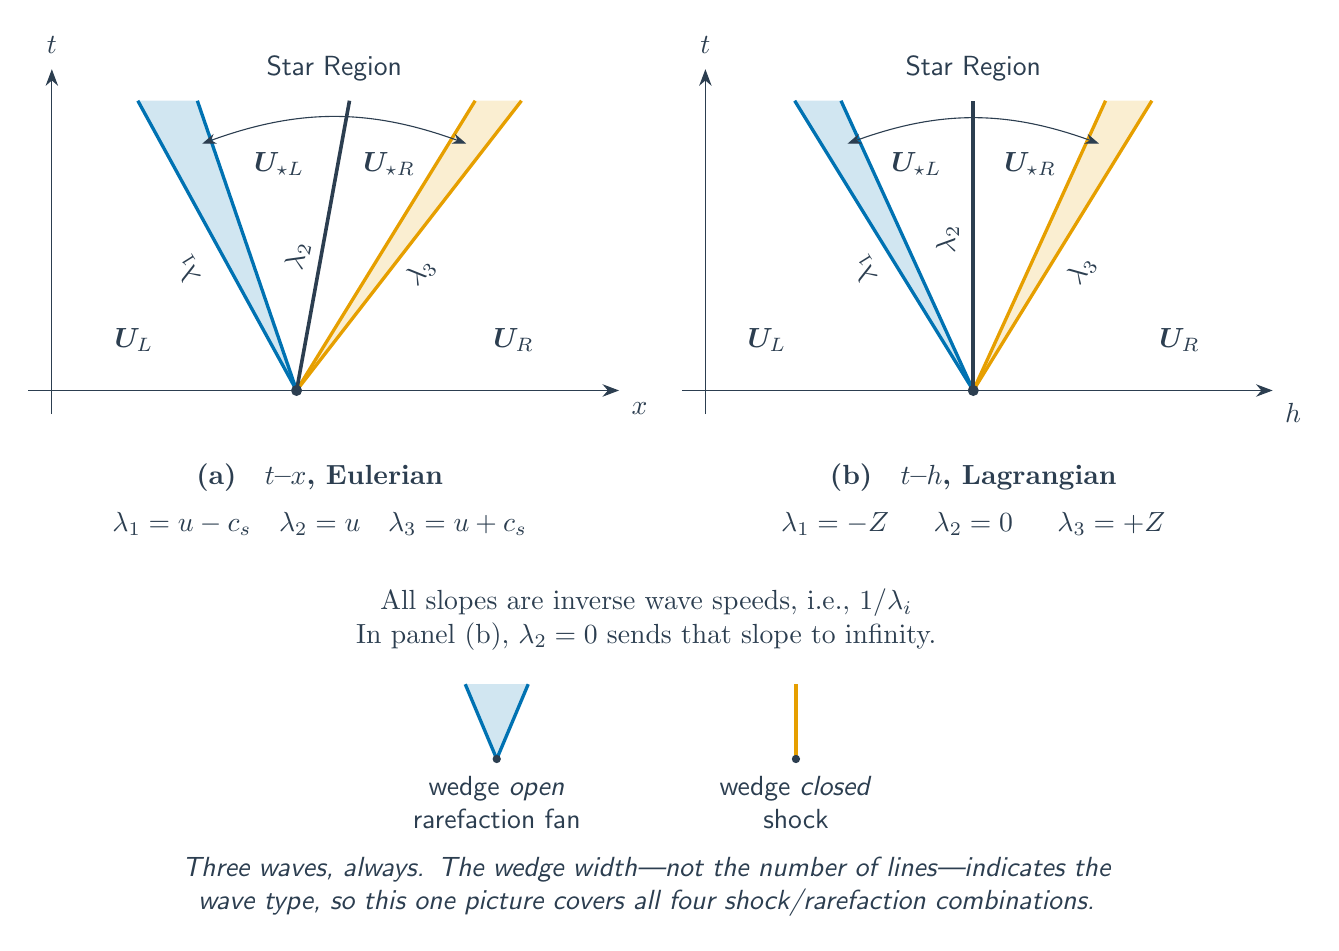
\begin{tikzpicture}[font=\sffamily, text=slate,
    declare function={
      T(\t) = \t*3.2;                    % cm per unit t  (both panels)
      Xa(\x) = (\x+1.85)*1.68;           % panel (a): x = -1.85 at 0
      Xb(\h) = (\h+2.025)*1.68 + 8.30;   % panel (b): h = -2.025 at 8.30
    }]

% ================= PANEL (a):  t -- x,  Eulerian =================
  % wedge tints (drawn first)
  \fill[oiblue!18]   ({Xa(0)},{T(0)}) -- ({Xa(-1.20)},{T(1.15)})
      -- ({Xa(-0.75)},{T(1.15)}) -- cycle;
  \fill[oiorange!18] ({Xa(0)},{T(0)}) -- ({Xa(1.35)},{T(1.15)})
      -- ({Xa(1.70)},{T(1.15)}) -- cycle;

  % wedge edges, contact
  \draw[edgeL]   ({Xa(0)},{T(0)}) -- ({Xa(-1.20)},{T(1.15)});
  \draw[edgeL]   ({Xa(0)},{T(0)}) -- ({Xa(-0.75)},{T(1.15)});
  \draw[edgeR]   ({Xa(0)},{T(0)}) -- ({Xa(1.35)},{T(1.15)});
  \draw[edgeR]   ({Xa(0)},{T(0)}) -- ({Xa(1.70)},{T(1.15)});
  \draw[contact] ({Xa(0)},{T(0)}) -- ({Xa(0.40)},{T(1.15)});
  \fill[slate]   ({Xa(0)},{T(0)}) circle (2.0pt);

  % region labels
  \node[reg] at ({Xa(-1.23)},{T(0.2)}) {$\bm{U}_L$};
  \node[reg] at ({Xa(-0.131)},{T(0.9)}) {$\bm{U}_{\star L}$};
  \node[reg] at ({Xa(0.700)}, {T(0.9)}) {$\bm{U}_{\star R}$};
  \node[reg] at ({Xa(1.64)}, {T(0.2)}) {$\bm{U}_R$};

  % wave labels -- ONE per wave, in the middle of the wedge
  \node[wlab, rotate=122, anchor=south] at ({Xa(-0.7)},{T(0.52)})
      {$\lambda_1$};
  \node[wlab, rotate=78.14, anchor=south] at ({Xa(0.15)},{T(0.52)})
      {$\lambda_2$};
  \node[wlab, rotate=48.25, anchor=north] at ({Xa(0.83)},{T(0.52)})
      {$\lambda_3$};

  % star-region sweep
  \draw[sweep] ({Xa(-0.7125)},{T(0.98)}) to[bend left=20] ({Xa(1.2825)},{T(0.98)});
  \node[wlab, anchor=south] at ({Xa(0.285)},{T(1.15)+0.16}) {Star Region};

  % axes
  \draw[axis] (-0.30,0) -- ({Xa(2.20)+0.40},0) node[below right=1pt] {$x$};
  \draw[axis] (0,-0.30) -- (0,{T(1.15)+0.40}) node[above=2pt] {$t$};
  \node[panel, anchor=north] at ({Xa(0.175)},-0.80) {(a)\;\; $t$--$x$, Eulerian};
  \node[reg, anchor=north] at ({Xa(0.175)},-1.42)
      {$\lambda_1 = u-c_s$\quad $\lambda_2 = u$\quad $\lambda_3 = u+c_s$};

% ================= PANEL (b):  t -- h,  Lagrangian =================
  \fill[oiblue!18]   ({Xb(0)},{T(0)}) -- ({Xb(-1.35)},{T(1.15)})
      -- ({Xb(-1.00)},{T(1.15)}) -- cycle;
  \fill[oiorange!18] ({Xb(0)},{T(0)}) -- ({Xb(1.00)},{T(1.15)})
      -- ({Xb(1.35)},{T(1.15)}) -- cycle;

  \draw[edgeL]   ({Xb(0)},{T(0)}) -- ({Xb(-1.35)},{T(1.15)});
  \draw[edgeL]   ({Xb(0)},{T(0)}) -- ({Xb(-1.00)},{T(1.15)});
  \draw[edgeR]   ({Xb(0)},{T(0)}) -- ({Xb(1.00)},{T(1.15)});
  \draw[edgeR]   ({Xb(0)},{T(0)}) -- ({Xb(1.35)},{T(1.15)});
  \draw[contact] ({Xb(0)},{T(0)}) -- ({Xb(0)},{T(1.15)});
  \fill[slate]   ({Xb(0)},{T(0)}) circle (2.0pt);

  \node[reg] at ({Xb(-1.560)},{T(0.2)}) {$\bm{U}_L$};
  \node[reg] at ({Xb(-0.430)},{T(0.9)}) {$\bm{U}_{\star L}$};
  \node[reg] at ({Xb(0.430)}, {T(0.9)}) {$\bm{U}_{\star R}$};
  \node[reg] at ({Xb(1.560)},{T(0.2)}) {$\bm{U}_R$};

  \node[wlab, rotate=122, anchor=south] at ({Xb(-0.7)},{T(0.52)})
      {$\lambda_1$};
  \node[wlab, rotate=90, anchor=south] at ({Xb(-.05)},{T(0.6)})
      {$\lambda_2$};
  \node[wlab, rotate=54.67, anchor=north] at ({Xb(0.7)},{T(0.52)})
      {$\lambda_3$};

  \draw[sweep] ({Xb(-0.95)},{T(0.98)}) to[bend left=20] ({Xb(0.95)},{T(0.98)});
  \node[wlab, anchor=south] at ({Xb(0)},{T(1.15)+0.16}) {Star Region};

  \draw[axis] ({Xb(-2.025)-0.30},0) -- ({Xb(2.025)+0.40},0)
      node[below right=1pt] {$h$};
  \draw[axis] ({Xb(-2.025)},-0.30) -- ({Xb(-2.025)},{T(1.15)+0.40})
      node[above=2pt] {$t$};
  \node[panel, anchor=north] at ({Xb(0)},-0.80) {(b)\;\; $t$--$h$, Lagrangian};
  \node[reg, anchor=north] at ({Xb(0)},-1.42)
      {$\lambda_1 = -Z$\quad\; $\lambda_2 = 0$\quad\; $\lambda_3 = +Z$};

% ---- slope convention: lambda is a SPEED, the drawn slope is its reciprocal --
  \node[reg, anchor=north, align=center] at (7.55,-2.40)
      {All slopes are inverse wave speeds, i.e., $1/\lambda_i$\\
       In panel (b), $\lambda_2 = 0$ sends that slope to infinity.};

% ================= LEGEND: what the wedge width means =================
  \begin{scope}[shift={(7.55,-4.68)}]
    % open wedge -> rarefaction
    \fill[oiblue!18] (-1.90,0) -- (-2.30,0.95) -- (-1.50,0.95) -- cycle;
    \draw[edgeL] (-1.90,0) -- (-2.30,0.95);
    \draw[edgeL] (-1.90,0) -- (-1.50,0.95);
    \fill[slate] (-1.90,0) circle (1.5pt);
    \node[wlab, anchor=north, align=center] at (-1.90,-0.12)
        {wedge \emph{open}\\ rarefaction fan};
    % closed wedge -> shock
    \draw[edgeR] (1.90,0) -- (1.90,0.95);
    \fill[slate] (1.90,0) circle (1.5pt);
    \node[wlab, anchor=north, align=center] at (1.90,-0.12)
        {wedge \emph{closed}\\ shock};
    \node[wlab, anchor=north, text width=13.5cm, align=center] at (0,-1.15)
        {\emph{Three waves, always. The wedge width---not the number of lines---indicates
         the wave type, so this one picture covers all four shock/rarefaction
         combinations.}};
  \end{scope}

\end{tikzpicture}
\end{document}
